\RequirePackage{fix-cm}
\documentclass[smallextended]{svjour3}
\smartqed

\usepackage{bbm}
\usepackage{cite}
\usepackage{tikz}
\usepackage{float}
\usepackage{amsmath}
\usepackage{graphicx}
\usepackage{enumitem}
\usepackage{changepage}
\usepackage[utf8]{inputenc}

% Command redefinitions
\let\origref\ref
\renewcommand{\ref}[1]{(\origref{#1})}

\journalname{Journal of Global Optimization}


\begin{document}
\title{Adaptive nested optimization scheme for multidimensional global search}

\author{Victor Gergel       \and
        Vladimir Grishagin  \and
        Alexander Gergel
}

%\authorrunning{Short form of author list} % if too long for running head

\institute{Department of Software, Nizhni Novgorod State University, pr. Gagarina, 23, 603950, Nizhni Novgorod, Russia \\
           \\
           V. Gergel \at
              \email{gergel@unn.ru}
           \and
           V. Grishagin \at
              \email{vagris@unn.ru}
           \and
           A. Gergel \at
              \email{gergelm@unn.ru} \\
           \\
           Tel: +7-831-462-33-56
}

\date{Received: date / Accepted: date}
% The correct dates will be entered by the editor


\maketitle

\begin{abstract}
Methods for solving the multidimensional multiextremal optimization problems using the nested optimization scheme are considered. A novel approach for solving the multidimensional multiextremal problems based on the adaptive nested optimization has been proposed. This approach enables to develop methods of the global optimum search which are more efficient in comparison with the ones on the base of the traditional nested optimization scheme. The new approach provides advantages due to better usage of the information on the problem in the course of optimization. A general scheme of a adaptive nested optimization is described. A theoretical substantiation of the method convergence is given for the case when for solving the univariate subproblems within the nested scheme an information algorithm of global search is used. Results of numerical experiments on the well-known classes of the test multiextremal functions confirming the efficiency of the proposed scheme are presented.

\keywords{Multidimensional multiextremal optimization \and Global search algorithms \and Dimensionality reduction \and Adaptive nested optimization scheme}
\end{abstract}


\section{Introduction}
\label{intro}
In the present article, methods for solving multiextremal problems widespread in the real life applications are considered. The increasing complexity of mathematical models for more adequate description of objects, phenomena, and systems under study results in a significant increase of the complexity in analysis of  these models. Numerical experiments become the primary tool for such an analysis. The increasing complexity of the problems results in the necessity of a purposeful selection of the variants in the process of the optimal solution search. The essence of the purposeful selection consists in eliminating from further consideration many obviously unpromising cases on the base of the analysis of a small portion of the variants in order to concentrate further search in the subdomains containing the best variants. However, the development of the efficient optimization algorithms in the multidimensional case is labor-consuming often. A possible way in this situation consists in applying different schemes of dimensionality reduction for the development of the global search methods.

The multidimensional multiextremal (\textit{global}) optimization problem without constraints can be defined as a problem of finding the minimal value of a real function $\varphi(x)$
%
\begin{equation}
\label{eq:1}
\varphi(y^*) = \min \{ \varphi(y): y \in D \},
\end{equation}
%
and its global minimizer $y^* \in D$, where
%
\begin{equation}
\label{eq:2}
D = \{ y \in \mathbbm{R}^N : y_i \in [a_i, b_i],  1 \leq i \leq N \}
\end{equation}
%
is the search domain, which  is a hyperparallelepiped in the $N$-dimensional Euclidean space $\mathbbm{R}^N$.

The global optimization problems are the subject of the extensive research (see, for example, comprehensive bibliography in \cite{Ref4, Ref5, Ref14, Ref15, Ref16, Ref22, Ref23, Ref24, Ref33, Ref36, Ref37, Ref38, Ref39}). At the same time, these problems are very computation-consuming. Thus, if  for the solution search  the method of full scanning the nodes of a uniform grid is used with the accuracy $\varepsilon > 0$ for each coordinate, the total number of the grid nodes in the search domain can be estimated as
%
\begin{equation*}
K = K(\varepsilon) \approx \prod\limits_{j = 1}^N \big[ (b_j - a_j) / \varepsilon \big].
\end{equation*}
%
The decrease of the computational costs is possible only thanks to the highly efficient global search algorithms, which generate the dense grids in the vicinity of the sought minimum of the minimized function only. The design of such efficient algorithms directly for the multidimensional case is a rather complex problem. As a result, using for this goal various \textit{dimensionality reduction schemes} is one of the directions in the field of global optimization. Within the framework of this direction, the following three main approaches could be outlined:

The first dimensionality reduction method is based on the well-known fundamental property, according to which an $N$-hyperparallelepiped from~\ref{eq:2} and the interval of the real axis $[0, 1]$ are the sets of equal cardinality, and the interval $[0, 1]$ can be mapped onto the hyperparallelepiped $D$ unambiguously and continuously (see \cite{Ref1, Ref30, Ref36}). The mappings of this kind are usually referred to as Peano \textit{evolvents} or curves.

Assume $y(x), x \in [0, 1]$, to be a Peano curve and the function $\varphi(y)$ from~\ref{eq:1} to be a continuous one. Then, the optimization problem for a multidimensional function $\varphi(y)$ can be reduced to a problem of optimization of a one-dimensional reduced function $\varphi(y(x))$
%
\begin{equation*}
\varphi(y(x^*)) = \min \{ \varphi(y(x)): x \in [0, 1] \} = \min \{ \varphi(y): y \in D \}.
\end{equation*}
This approach has served a basis for the development of many efficient multidimensional global search algorithms (see \cite{Ref9, Ref11, Ref13, Ref30, Ref34, Ref36}).

In the framework of the second approach, the search domain is divided into the subdomains by means of a partition strategy, each subdomain is estimated from the point of view of its importance, or prospectivity for continuation of the search and the next iteration point is chosen in the subdomain of maximal importance. This approach is close to univariate scheme of characteristical algorithms \cite{Ref11} and the methods based on multidimensional partitioning are presented, for instance, in \cite{Ref17, Ref19, Ref20, Ref21, Ref22, Ref23, Ref24}.

Finally, the well-known approach based on the usage of the one-dimensional optimization methods for solving the multidimensional optimization problems  consists in the application of the \textit{nested optimization scheme}. According to this scheme, the solving of a multidimensional optimization problem could be obtained by means of solving  a sequence of the recursively nested one-dimensional problems (see, for example \cite{Ref2, Ref3, Ref8, Ref12, Ref25, Ref28, Ref31, Ref36}). The core of this approach is the relation
\begin{equation}
\label{eq:3}
\min_{y \in D} \varphi(y) = \min_{y_1 \in [a_1, b_1]} \dots \min_{y_N \in [a_N, b_N]} \varphi(y_1, \dots, y_N).
\end{equation}

According to~\ref{eq:3} the solving of a multidimensional multiextremal optimization problem is reduced to the solving of the one-dimensional problem:
%
\begin{equation}
\label{eq:4}
\varphi^* = \min_{y \in D} \varphi(y) = \min_{y_1 \in [a_1, b_1]} \widetilde{\varphi}_1(y_1),
\end{equation}
%
where
%
\begin{equation}
\label{eq:5}
\widetilde{\varphi}_i(y_i) = \varphi_i(y_1, \dots, y_i) = \min_{y_1 \in [a_{i + 1}, b_{i + 1}]} \varphi_{i + 1}(y_1, \dots, y_i, y_{i + 1}), 1 \leq i \leq N,
\end{equation}
%
\begin{equation}
\label{eq:6}
\varphi_N(y_1, \dots, y_N) = \varphi(y_1, \dots, y_N).
\end{equation}
%
The one-dimensional function $\widetilde{\varphi}_1(y_1)$ introduced in~\ref{eq:4} is constructed according to general recursive rule~\ref{eq:5}: in order to calculate the value $\widetilde{\varphi}_1(y_1)$ for given value of the variable $y_1 = \hat{y}_1$ it is necessary to perform the minimization of the function
\begin{equation*}
\widetilde{\varphi}_2(y_2) = \varphi_2(\hat{y}_1, y_2).
\end{equation*}
%
When performing this optimization, the function $\widetilde{\varphi}_2$ is a one-dimensional one as well since the value of the variable $y_1$ is predefined and fixed. Next, in turn, in order to calculate the value $\widetilde{\varphi}_2(y_2)$ at the point $y_2 = \hat{y}_2$ it is necessary to perform the minimization of the univariate function
\begin{equation*}
\widetilde{\varphi}_3(y_3) = \varphi_3(\hat{y}_1, \hat{y}_2, y_3),
\end{equation*}
%
etc.

The scheme~\ref{eq:4}--\ref{eq:6} in the case of  the Lipschitzian one-dimensional functions $\widetilde{\varphi}_i$ combined with the one-dimensional algorithms \cite{Ref7, Ref25, Ref32, Ref34, Ref35, Ref36} has served as the basis for designing  a number of the multidimensional methods \cite{Ref3, Ref12, Ref25, Ref26, Ref36}.

Concluding the characterization of the nested optimization scheme, it should be noted that this approach to the design of the multidimensional methods has also a number of disadvantages. When solving the particular subproblem~\ref{eq:5} the information on the behavior of the objective function obtained during solving other subproblems is not used in any way. This is the fundamental cause of the loss in the efficiency of the nested scheme. On the one hand, this makes the computational scheme simpler because allows to avoid storing and processing large amount of information. On the other hand, the refusal from the information worsens the search process planning quality.
Besides, when using this scheme, the precision in the termination condition providing the termination of any recursively nested one-dimensional problem like~\ref{eq:5} should be defined a priori. If the accuracy appears to be not enough, it is required to repeat the solving of the problem as a whole from the beginning with an increased precision. At the same time, the use of too high precision can result in an essential increase in the global search duration, and breaking the computations before the termination condition is satisfied (because of exceeding of the feasible computation time) in this case can lead to the case when the estimate of the sought solution is obtained in some subdomain of the search domain $D$ only.

The rest of the paper is organized as follows. Section~\origref{sec:2} describes a new generalization of the nested optimization scheme. Section~\origref{sec:3} is devoted to the theoretical substantiation of the new scheme concerning convergence properties. Section~\origref{sec:4} contains results of computational experiments. The last section gives a succinct summary of the paper.

\section{Adaptive nested optimization  scheme}
\label{sec:2}
Let us give a generalization of the basic scheme of dimensionality reduction~\ref{eq:3}--\ref{eq:6} allowing to overcome some disadvantages of the approach mentioned above. The essence of this generalization consists in the elimination of the principle of a strict subordination for the minimization problems of the one-dimensional functions $\widetilde{\varphi}_i(y_i), 1 \leq i \leq N$, generated within the framework of the nested optimization scheme. In the new approach all these problems are supposed to be solved simultaneously.

The preliminary description of the proposed generalization is as follows.

Let us introduce the following notation for brevity
\begin{equation}
\label{eq:7}
\nu_i = (y_1, \dots, y_i), 1 \leq i \leq N.
\end{equation}

Then, the one-dimensional functions $\widetilde{\varphi}_i(y_i), 1 < i \leq N$, generated within the framework of the nested optimization scheme can be rewrote in the form
\begin{equation}
\label{eq:8}
\widetilde{\varphi}_i(y_i) = \varphi_i(\nu_{i - 1}, y_i), 1 < i \leq N,
\end{equation}
%
where the vector $\nu_{i - 1}$ is a fixed one.

Let us describe in more details the procedure of computations for the initial (basic) scheme of dimensionality reduction.

At every global search iteration $i, 1 \leq i \leq k$, the optimization algorithm begins its computations from a one-dimensional function of the first level $\widetilde{\varphi}_1(y_1)$. The algorithm selects a current search point $y_1 = \hat{y}_1$ taking into account the search information obtained already. In order to get the function value $\widetilde{\varphi}_1(y_1)$ at this point, a new one-dimensional function $\varphi_2(\hat{y}_1, y_2)$ to be minimized is generated. To do so, the algorithm should suspend the minimization of the function $\widetilde{\varphi}_1(y_1)$ and start minimizing the function $\varphi_2(\hat{y}_1, y_2)$. In the optimization process of the function $\varphi_2(\hat{y}_1, y_2)$, the algorithm generates a sequence of the points
\begin{equation*}
\{ y_2^j, 1 \leq j \leq k \},
\end{equation*}
%
for each of which it is necessary to execute the minimization of the third level $\varphi_3(\hat{y}_1, \hat{y}_2, y_3)$ in the same strict order: when determining the next search point before the transition to the next search iteration, the solving of a one-dimensional problem of the next dimensionality reduction level should be carried out first. This process should be fulfilled recursively until the last $N^{\text{th}}$ level. The resulting hierarchical scheme of generating and solving the one-dimensional problems is presented in Fig.~\origref{fig:1}.

\begin{figure}[H]
\centering
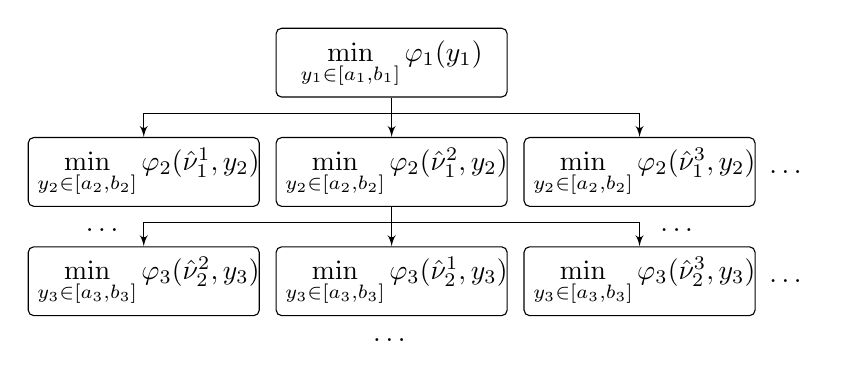
\begin{tikzpicture}
\usetikzlibrary{arrows,positioning,calc}
\tikzset{
  task/.style = {draw, text width=27mm, text height=3mm, rectangle, rounded corners=2pt, align=center},
  arrow/.style ={->, >=latex'}
}

\node[task] (task11) {$\min\limits_{y_1 \in [a_1, b_1]}\varphi_1(y_1)$};

\node[task, below=5mm of task11] (task22) {$\min\limits_{y_2 \in [a_2, b_2]}\varphi_2(\hat{\nu}_1^2, y_2)$};
\node[task, left=2mm of  task22] (task21) {$\min\limits_{y_2 \in [a_2, b_2]}\varphi_2(\hat{\nu}_1^1, y_2)$};
\node[task, right=2mm of task22] (task23) {$\min\limits_{y_2 \in [a_2, b_2]}\varphi_2(\hat{\nu}_1^3, y_2)$};

\node[task, below=5mm of task22] (task32) {$\min\limits_{y_3 \in [a_3, b_3]}\varphi_3(\hat{\nu}_2^1, y_3)$};
\node[task, left=2mm of  task32] (task31) {$\min\limits_{y_3 \in [a_3, b_3]}\varphi_3(\hat{\nu}_2^2, y_3)$};
\node[task, right=2mm of task32] (task33) {$\min\limits_{y_3 \in [a_3, b_3]}\varphi_3(\hat{\nu}_2^3, y_3)$};

\draw[arrow] (task11.south) -- ++(0,-0.2) -|  (task21.north);
\draw[arrow] (task11.south) -- ++(0,-0.2) -|  (task22.north);
\draw[arrow] (task11.south) -- ++(0,-0.2) -|  (task23.north);

\draw[arrow] (task22.south) -- ++(0,-0.2) -|  (task31.north);
\draw[arrow] (task22.south) -- ++(0,-0.2) -|  (task32.north);
\draw[arrow] (task22.south) -- ++(0,-0.2) -|  (task33.north);

\node at ($ (task31.north) + (-0.5,  0.2) $) {$\dots$};
\node at ($ (task33.north) + ( 0.5,  0.2) $) {$\dots$};
\node at ($ (task32.south) + ( 0.0, -0.3) $) {$\dots$};
\node[right=0.5mm of task23] {$\dots$};
\node[right=0.5mm of task33] {$\dots$};

\end{tikzpicture}
\caption{\label{fig:1}The hierarchical scheme of generating and solving the one-dimensional problems in the nested optimization scheme}
\end{figure}

The functions generated during the optimization process have a strict hierarchical structure of subordination in the form of a tree. The structure of this tree changes dynamically in the course of solving the multidimensional task. The computation of the function value $\varphi_i(\hat{\nu}_{i - 1}, y_i)$ of the $i^{\text{th}}$ level, $1 \leq i < N$, at some point   requires solving all problems in one of the subtrees of the $(i + 1)^{\text{th}}$ level. The functions $\varphi_N(\hat{y}_{N - 1}, y_N)$ of the $N^{\text{th}}$ level are the leaves of the problem tree, their values are the values of the objective function $\varphi(y), y \in D$, and are computed directly without the nested optimization.

The \textit{proposed generalization of the basic scheme} of the dimensionality reduction consists in the elimination of the strict order of the subproblem solving according to their hierarchy in the problem tree, when the solving of the problem of the $i^{\text{th}}$ level, $1 \leq i < N$, does not require the complete  solving of the nested problems of the $(i + 1)^{\text{th}}$ level. Within the framework of the novel approach all generated problems are considered simultaneously and are equal in rights. The proposed approach will be hereinafter referred to as \textit{the adaptive nested optimization scheme}.

For description of the approach, let us renumber problems~\ref{eq:5} in the following way. Since the nested optimization scheme starts from the solving of the problem
\begin{equation}
\label{eq:9}
\min_{y_1 \in [a_1, b_1]} \varphi_1(y_1),
\end{equation}
%
let us assign to this problem the index $l = 1$. The solving of this problem begins with the computation of the function $\widetilde{\varphi}_1(y_1)$ at some point $\hat{y}_1$ that generates the problem
\begin{equation*}
\min_{y_2 \in [a_2, b_2]} \varphi_2(\hat{y}_1, y_2),
\end{equation*}
%
to which the index $l = 2$ is assigned, etc.

In general, when $Q \leq 1$ subproblems~\ref{eq:5} have been initiated already, the index $Q + 1$ is assigned to a newly generated subproblem, and the number of subproblems $Q$ is incremented by $1$.

Thus, at every moment of execution of the nested optimization scheme there is a set $F_Q$ consisting of the problems of the kind
\begin{equation}
\label{eq:10}
\min_{x \in [a, b]} f_l(x), 1 \leq l \leq Q,
\end{equation}
%
where the index $l$ is connected with a recursion level, i.e., with the coordinate number $i, 1 \leq i \leq N$, which this problem belongs to. In this case $x = y_i$, and the search domain $[a, b] = [a(l), b(l)]$ is the interval $[a_i, b_i]$. When $i = 1$, $f_l(x) = \varphi_1(y_1)$. If $i > 1$, then the index $l$ is also connected with the vector $\nu_{i - 1} = \nu_{i - 1}(l)$ and $f_l(x) = \varphi_i(\nu_{i - 1}, y_i)$. Moreover, any problem~\ref{eq:10} except the problem $f_l(x)$ is associated with the ``parent'' one, i.e., with a problem which has generated it.

Let us designate the operation of the computation of the objective function value at a given point of the search domain as the trial. Consider the methods, which generate during solving the problem~\ref{eq:10} the sequence of trial coordinates $x_l^1, x_l^2, \dots, x_l^k, \dots$ and the sequence of the trial results (the function values) $z_l^1, z_l^2, \dots, z_l^k, \dots$, where $z_l^j = f_l(x_l^j), j \geq 1$. After completing $k \geq 1$ trials the set of the search information is formed
\begin{equation}
\label{eq:11}
\omega_l^k = \big\{ (x_l^j, z_l^j, \lambda_l^j): 1 \leq j \leq k \big\},
\end{equation}
%
where $\lambda_l^j, 1 \leq j \leq k$, are the indices of the problems generated for the computation of the values $z_l^j, 1 \leq j \leq k$. Within the framework of the multidimensional scheme, it is reasonable to form the search information separately for each problem of the family $F_Q$ under solving. As a complete set of information for the multidimensional problem being solved one can consider the set
\begin{equation*}
\Omega_Q = \big\{ \omega_l^{k(l)}, 1 \leq l \leq Q \big\},
\end{equation*}
%
where $k(l), 1 \leq l \leq Q$, is the number of the search information elements for the problem with the index $l$. It is important to note that the values $z_l^j, 1 \leq j \leq k(l)$, in the search information for the function of the level less than $N$ may vary since these values are the estimates of the minimum values of the functions $f_l$, and these estimates may be refined during the computations.

Note that in traditional nested optimization scheme, in the course of solving a problem~\ref{eq:10} the information on the particular sets~\ref{eq:11} is used only while in the adaptive generalization the full set of information~\ref{eq:12} is taken into consideration.

Before the detailed description of the general adaptive scheme let us introduce some auxiliary terms. When a univariate subproblem generates for computing the value of its objective function a subproblem of the next level we will call the generating subproblem as parental one, or just a parent, and the generated subproblem as the upper one. Obviously, the subproblem~\ref{eq:9} of the first level can be parental only and subproblems of the level $N$ have no upper levels. Let us juxtapose to the subproblem with the index $l$ from the set $F_Q$ (except the subproblem~\ref{eq:9} with the index $l = 1$) the number $\pi(l)$ of its parent and the number $\rho(l)$ of a recursion level (number of coordinate) which this subproblem belongs to. Moreover, let us consider a point $x_l^j$ being $j$-th trial in the course of solving the problem~\ref{eq:10} with the number $l$ and connect with it the number $\lambda_l^j$ of a subproblem generated for computing the function value at this point. Let us introduce as well the designation $\varphi_l^*$ for the current minimal value of objective function $f_l$ from~\ref{eq:10}.

\begin{enumerate}[label=\bfseries Step \arabic*., leftmargin=*]
  \item \textbf{Initialization.}
  \begin{enumerate}[label=\arabic{enumi}.\arabic*., leftmargin=-2em]
    \item Set the number of subproblems of the nested scheme $Q = 0$ and the number of coordinate level $l = 1$. Accept the level number $i = 1$. Choose a point $x_1^1$ in the interval $[a_1, b_1]$ as the starting point of solving the univariate subproblem~\ref{eq:9}. Increase $Q$ by $1$ and include this problem in the set $F_Q$ with the index $l = 1$.

    \item For calculating at the level $i$ the value of the objective function at the point $x_i^1$, pass to the next coordinate ($i = i + 1$) for solving the univariate subproblem
    \begin{equation}
      \label{eq:12}
      \min_{y_i \in [a_i, b_i]} \varphi_i(\hat{\nu}_{i - 1}, y_i),
    \end{equation}
    where the components of the vector $\hat{\nu}_{i - 1} = (\nu_1, \dots, \nu_{i - 1})$ are constants. Namely, $\nu_j = x_j^1, 1 \leq j \leq i - 1$.

    \item Choose a point $x_i^1$ in the interval $[a_i, b_i]$ as the starting point for solving the subproblem~\ref{eq:12}. Increase $Q$ by $1$ and include this problem in the set $F_Q$ with the index $l = i$.

    \item Repeat operations 1.2 and 1.3 up to reaching the level $i = N$. At this level calculate the value $z_N^1$ of objective $\varphi(y)$ function from~\ref{eq:1} at the point $y = (x_1^1, \dots, x_N^1)$ instead of generating a new univariate subproblem.

    \item For all subproblems from $F_Q$ with numbers $l, 1 \leq l \leq Q$:
    \begin{enumerate}[label=\arabic{enumi}.\arabic{enumii}.\arabic*., leftmargin=*]
      \item If $l \leq N$, then set $\lambda_l^1 = l + 1$ (for the $l = N$ number $\lambda_l^1$ is undefined).
      \item Accept $z_l^1 = z_N^1$, $k(l) = 1$, and form the sets of search information $\omega_l^{k(l)} = \{( x_l^1, z_l^1, \lambda_l^1 )\}$ (except $l = N$ where $\omega_l^{k(l)} = \{( x_l^1, z_l^1 )\}$).
      \item Specify current minimal value $\varphi_l^* = z_l^1$, $\rho(l) = l$, and for $l > 1$ accept $\pi(l) = l - 1$.
    \end{enumerate}
  \end{enumerate}

  \vspace{3 mm}
  \item \textbf{Main procedure.}
  \begin{adjustwidth}{-4em}{}
    %Add margin%
    Let there be $Q$ subproblems~\ref{eq:10} for which sets~\ref{eq:11} have been formed and the values $\pi(l)$, $\rho(l)$, $\varphi_l^*$ have been determined. The next iteration of the adaptive scheme is executed in accordance with the following rules.
  \end{adjustwidth}
  \begin{enumerate}[label=\arabic{enumi}.\arabic*., leftmargin=-2em]
    \item Choice of univariate subproblem.
    \begin{enumerate}[label=\arabic{enumi}.\arabic{enumii}.\arabic*., leftmargin=*]
      \item Assign to each subproblem~\ref{eq:10} with the index $l, 1 \leq l \leq Q$, the value $\widetilde{R}(l)$ called the characteristic of this subproblem.
      \item Find among the subproblems~\ref{eq:10} a subproblem with index $\sigma, 1 \leq \sigma \leq Q$, which the maximal characteristic corresponds to
      \begin{equation}
      \label{eq:13}
      \widetilde{R}(\sigma) = \max \big\{ \widetilde{R}(l): 1 \leq l \leq Q \big\}.
      \end{equation}
    \end{enumerate}
    \item New iteration.
    \begin{enumerate}[label=\arabic{enumi}.\arabic{enumii}.\arabic*., leftmargin=*]
      \item Set $l = \sigma, i = \rho(\sigma)$ and determine a point $x_l^{k(l) + 1}$ of the next trial in the subproblem $\sigma$ taking into account the search information~\ref{eq:11}. If $i < N$, then accept $\lambda_l^{k(l) + 1} = Q + 1$.

      \item If $i = N$, then calculate the value $z_l^{k(l) + 1} = \varphi(\hat{\nu}_{i - 1}, x_l^{k(l) + 1})$ where the vector $\hat{\nu}_{i - 1}$ has been determined in preceding parental subproblems. Renew the current estimation of minimum $\varphi_l^*$ and the search information adding the pair $(x_l^{k(l) + 1}, z_l^{k(l) + 1})$ to the set~\ref{eq:11} and incrementing $k(l)$ by $1$. Then pass to Substep 2.3. In the opposite case ($i < N$) go to 2.2.3.

      \item For calculating at the level $i$ the value of the objective function at the point $x_l^{k(l) + 1}$ take the next coordinate ($i = i + 1$) for solving a new univariate subproblem~\ref{eq:12} (the components of the vector $\hat{\nu}_{i - 1}$ are fixed). Increase $Q$ by $1$ and assign to the new subproblem the number $l = Q$ in the set $F_Q$.

      \item Choose a point $x_l^1$ in the interval $[a_l, b_l]$ as the starting point for solving the new subproblem~\ref{eq:12}. Define the set~\ref{eq:11} as empty one and assign $k(l) = 0$. Accept $\varphi_l^* = +\infty$, $\rho(l) = i$, $\lambda_l^1 = Q + 1$.

      \item If the subproblem $\sigma$ is parental for the current one, then set $\pi(l) = \sigma$, otherwise, $\pi(l) = Q - 1$. Go to 2.2.2.
    \end{enumerate}

    \item Renewing the search information in parental subproblems.
    \begin{enumerate}[label=\arabic{enumi}.\arabic{enumii}.\arabic*., leftmargin=*]
      \item Return to the parental subproblem: new $l = \pi(l)$.

      \item If the set $\omega_l^{k(l)}$ is empty or $l = \sigma$, then accept the current minimal value of subproblem with number $\lambda_l^{k(l)}$ as the objective function value $z_l^{k(l)}$ at the new trial point $x_l^{k(l)}$, include in the set $\omega_l^{k(l)}$ the triplet $\big( x_l^{k(l)}, z_l^{k(l)}, \lambda_l^{k(l)} \big)$, add unity to $k(l)$ and renew the estimate $\varphi_l^*$.

      \item Repeat operations 2.3.1 and 2.3.2, if $l \neq \sigma$. In the opposite case, go to 2.3.4.

      \item Accept $\mu = \pi(l)$ and pass to the parental subproblem: new $l = \pi(l)$.

      \item Find in the set $\omega_l^{k(l)}$ a triplet $\big( x_l^j, z_l^j, \lambda_l^j \big), 1 \leq j \leq k(l)$, for which $\lambda_l^j = \mu$ and replace $z_l^j$ with $\varphi_{\mu}^*$.

      \item If $\varphi_{\mu}^* < \varphi_l^*$, then replace $\varphi_l^*$ with $\varphi_{\mu}^*$ and go to 2.3.4. In the opposite case, complete the current iteration of the main procedure and return to Substep 2.1.

    \end{enumerate}
  \end{enumerate}
\end{enumerate}

Description of the adaptive nested optimization scheme has been completed.

In the algorithmic scheme presented above the decision rules for choice of starting points in univariate subproblems and for selection the best subproblem (characteristics $\widetilde{R}(l)$ in 2.2.1) are not defined. Generally speaking, this characteristic $\widetilde{R}(l)$ is determined by a one-dimensional method that are used for solving the subproblem $l$.

In the present research, the global search algorithm developed within the framework of the information approach (see \cite{Ref34, Ref35, Ref36}) has been applied for solving the one-dimensional problems~\ref{eq:10}. Let us show how this method forms the subproblem characteristic $\widetilde{R}(l)$. According to this algorithm, while solving a univariate problem~\ref{eq:10} the first trial is executed at some internal point of the interval $[a, b]$. For certainty, the starting point $x_l^1$ is considered to be the middle of the interval $[a, b]$ where the value $z_l^1 = f_l(x_l^1)$ is computed.

The choice of the point $x_l^{k + 1}, k > 1$ of any subsequent $(k + 1)$-th trial is determined by the following operations:
\begin{enumerate}[label=\bfseries Step \arabic*., leftmargin=0em, itemindent=*, itemsep=1em]
  \item Coordinates of the previous trials $x_l^1, x_l^2, \dots, x_l^k$ from~\ref{eq:11} and the ends of the interval $[a, b]$ are renumbered by subscripts in increasing order:
  \begin{equation}
  \label{eq:14}
  a = x_0 < x_1 < \dots < x_k < x_{k + 1} = b,
  \end{equation}
  %
  and the values $z_j = f_l(x_j), 1 \leq j \leq k$, are juxtaposed to them (besides $x_0$ and $x_{k + 1}$). Values $z_j, 1 \leq j \leq k$, are taken from the set~\ref{eq:11} because they are the corresponding outcomes $z_j, 1 \leq j \leq k$.

  \item For each interval $(x_{j - 1}, x_j), 1 \leq j \leq k + 1, k = k(l)$, a value $R(j)$ hereinafter called the characteristic of the interval is calculated as follows

  \begin{equation*}
  R(1) = 2m(x_1 - x_0) - 4z_1, j = 1,
  \end{equation*}
  %
  \begin{equation}
  \label{eq:15}
  R(j) = m(x_j - x_{j - 1}) + \frac{(z_j - z_{j - 1})^2}{m(x_j - x_{j - 1})} - 2(z_j + z_{j - 1}), 1 < j < k + 1,
  \end{equation}
  %
  \begin{equation*}
  R(k + 1) = 2m(x_{k + 1} - x_k) - 4z_k, j = k + 1
  \end{equation*}
  %

  \item The interval $(x_{t - 1}, x_t)$ with the index $t = t(l)$, which the maximal characteristic $R(t)$ corresponds to is selected, i.e.,
  \begin{equation}
  \label{eq:16}
  R(t) = \max \big\{ R(j): 1 \leq j \leq k + 1 \big\},
  \end{equation}
  %
  and the value $R(t)$ is accepted as the characteristic $\widetilde{R}(l)$ of the subproblem $l$.

  \item The next trial points in the interval with the maximal characteristic is calculated as
  \begin{equation}
  \label{eq:17}
  x^{k + 1} = \frac{x_t + x_{t - 1}}{2} - \frac{z_t - z_{t - 1}}{2m}, 1 < t < k + 1,
  \end{equation}
  \begin{equation*}
  x^{k + 1} = \frac{x_t + x_{t - 1}}{2}, t = 1, t = k + 1.
  \end{equation*}

  Here the value $m$ can be considered as an estimate of Lipschitz constant of the minimized function. It can be calculated adaptively on the base of the trial results as
  \begin{equation}
  \label{eq:18}
    m =
      \begin{cases}
      rM, & \quad M > 0, \\
       1, & \quad M = 0
      \end{cases}
  \end{equation}
  %
  where
  \begin{equation*}
  M = \max_{1 < i \leq k} \frac{|z_i - z_{i - 1}|}{x_i - x_{i - 1}},
  \end{equation*}
  %
  and $r > 1$ is a parameter of the method.

  The algorithm can be supplemented with a termination criterion:

  \item If
  \begin{equation}
  \label{eq:19}
  x_t - x_{t - 1} \leq \varepsilon,
  \end{equation}
  where $t$ from~\ref{eq:16} is the index of the interval with the maximal characteristic, then stop. In the opposite case, it is necessary to calculate $z_l^{k + 1} = f_l(x_l^{k + 1})$, to increment $k$ by $1$ and to pass to Step 1. Here $\varepsilon > 0$ is the predefined search accuracy (for the coordinates).
\end{enumerate}
The univariate method describes above belongs to the class of the characteristical global search algorithm (see \cite{Ref11, Ref36}). This class includes many well known one-dimensional multiextremal optimization methods, such as, for example, algorithms~\cite{Ref18, Ref25, Ref26, Ref32, Ref36} which can be embedded into the adaptive nested scheme as well.

Using the rule~\ref{eq:19} one can introduce a termination condition into the adaptive nested scheme. It can be either a ``strong'' criterion when~\ref{eq:19} is satisfied for all problems from the set $F_Q$ or a weaker one when the inequality~\ref{eq:19} holds for the problem~\ref{eq:9} only.


\section{Convergence of the adaptive nested optimization scheme}
\label{sec:3}
In order to prove the convergence of the proposed approach, let us note first that in the novel generalized multistep scheme \textit{the current estimate of the minimum value} of the function $\widetilde{\varphi}_{i + 1}(y_{i + 1})$ determined on the base of the completed global search iterations is used as the sought function value $\widetilde{\varphi}_i(y_i)$. The estimates used can be refined during the computations. However, the estimates may differ from the values obtained by the exact solving of problems~\ref{eq:4} essentially. More strictly, one can say that in the global search the computations deal not with the ``exact'' one-dimensional functions $\widetilde{\varphi}_i(y_i), 1 \leq i < N$, but with the approximations $\widetilde{\psi}_i(y_i), 1 \leq i < N$, of these ones. Therefore, after completing the optimization, some estimate $\psi^*$ of the exact solution $\varphi^*$ from~\ref{eq:4} will be obtained. In this connection, an important question on the nearness of the estimates $\psi^*$ and $\varphi^*$ arises. It is worth noting that the approximate computations of the one-dimensional function values are inherent in the basic nested optimization scheme as well (see \cite{Ref34, Ref35}). For this scheme, the following theorem is true:

\newtheorem{mytheorem}{Theorem}
\begin{mytheorem}
\label{th:1}
% Remove italic
(see \cite{Ref34}) Let the functions $\varphi_i(\nu_i)$ be the Lipschitzian ones with the constants $L_i$ for any $i$, $1 \leq i \leq N$. Then, the following assertion is true for the approximation $\psi^*$ obtained in the minimization of the function $\varphi(y), y \in D$, by the information algorithm using the basic scheme of nested optimization:
\begin{equation*}
\lim_{\varepsilon_i \to 0} \psi^* = \varphi^*,
\end{equation*}
if
\begin{equation*}
\varepsilon_{i + 1} = O(\varepsilon_i), 1 \leq i < N,
\end{equation*}
and besides, the inequality
\begin{equation}
\label{eq:20}
m_i \geq 2L_i + \theta, 1 \leq i < N, \theta > 0,
\end{equation}
holds after terminating the minimization for coordinate $y_i$ (i.e., after solving any problem~\ref{eq:10} with $l = l(i)$).
\end{mytheorem}

Here $m_i$ are estimates~\ref{eq:18} applied in the solving of subproblems~\ref{eq:10} for the corresponding coordinates $y_i$, $\varepsilon_i$ are the accuracies for the solutions of these problems in termination criterion~\ref{eq:19}, and $O(\varepsilon_i)$ are the infinitesimal in comparison with $\varepsilon_i$.

Theorem~\origref{th:1} is a theoretical substantiation of the applicability of the basic nested optimization scheme. At the same time, it could be considered as the justification of the convergence of the adaptive scheme as well if a ``strong'' termination condition is applied, i.e., when~\ref{eq:19} is satisfied for all one-dimensional subproblems. In this case, the order of computations is changed in the realization of the scheme only.

In the case of using the adaptive scheme with the ``weak'' termination condition the applicability of the theorem is limited. The one-dimensional problems $f_l(x), 1 \leq l \leq Q,$ of the family $F_Q$ from~\ref{eq:10} are considered simultaneously. A part of these ones (with large enough values of the minimized function $\varphi(y)$) may be never solved with the required accuracy $\varepsilon$. This is the initial idea for improvement efficiency of the adaptive scheme. As a result, the error of the calculations of the functions $\varphi_i(\nu_i)$ may appear to be considerable. This error may remain unchanged even when $\varepsilon$ tends to zero. In order to resolve this problem, one can note that actually there is no need in the exact calculation of the functions $\varphi_i(\nu_i)$ in all points of the feasible domain. The necessary requirement is the condition of the exact calculation of these functions in the nearness of the global minimum of the initial function $\varphi(y)$ only. Just because this requirement will be used further for the theoretical substantiation of the adaptive nested optimization scheme.

Let us represent the search information $\omega_l^{k(l)}, 1 \leq l \leq Q$, from~\ref{eq:11}--\ref{eq:12} obtained during the global search for the functions $f_l(x) = \varphi_i(\nu_i, x), 1 \leq l \leq Q$, where $x = y_i, i = i(l)$, in the form
\begin{equation}
\label{eq:21}
\omega_l^{k(l)} = \{ (y_{l, j}, z_{l, j}(\delta_{l, j}), \lambda_{l, j}): 1 \leq j \leq k(l) \},
\end{equation}
%
where $y_{l, j}, 1 \leq j \leq k(l)$, are the points of the completed $l$ search trials, the index $l$ corresponds to the index of the problem in the family $F_Q$, the index $j$ corresponds to the increasing order of the iteration points~\ref{eq:14} in the search information, $\delta_{l, k}, 1 \leq j \leq k(l)$, are the errors of the computation of the values $z_{l, j}, 1 \leq j \leq k(l)$, i.e.,
\begin{equation}
\label{eq:22}
(z_{l, j} - \varphi_{\lambda_{l, j}}(\nu_{\lambda_{l, j}}, y_{l, j})) \leq \delta_{l, j}.
\end{equation}
%
Remind (see~\ref{eq:9}) that $\lambda_{l, j}, 1 \leq j \leq k(l)$, are the indices of the problems from the family $F_Q$, which were generated to calculate the values $z_{l, j}, 1 \leq j \leq k(l)$. It is important to emphasize also that the errors $\delta_{l, j}, 1 \leq j \leq k(l)$, could appear to be different for different points $z_{l, j}, 1 \leq j \leq k(l)$.

The possibility to obtain the estimates of the global minimum of the initial function $\varphi(y), y \in D$, is defined by the conditions of the following theorem.

\begin{mytheorem}
\label{th:2}
Let the adaptive scheme using the information global search algorithm~\ref{eq:14}--\ref{eq:18} and the ``weak'' termination condition~\ref{eq:19} for problem~\ref{eq:9} with $\varepsilon = 0$ be applied to solving problem~\ref{eq:1}. If
\begin{enumerate}[label=\roman*)]
  \item the objective function $\varphi(y)$ of problem~\ref{eq:1} satisfies the Lipschitz condition with a finite constant $L > 0$ in domain~\ref{eq:2};

  \item starting from some search step, the inequality
  \begin{equation}
  \label{eq:23}
  m > 2L,
  \end{equation}
  for the estimates $m$ of Lipschitz constant from~\ref{eq:18} holds;

  \item for any function $f_l(x) = \varphi_i(\nu_i, x), 1 \leq l \leq Q, i = i(l)$, of the family $F_Q$ from~\ref{eq:10} the following conditions for the errors of the function values' calculation hold
  \begin{multline}
  \label{eq:24}
  \delta_{l, \tau} + \delta_{l, \tau - 1} \leq 2\varphi(y^*) + L(y_{l, \tau} - y_{l, \tau - 1}) - \\
  - (\varphi_{\lambda_{l, \tau}}(\nu_i, y_{l, \tau}) + \varphi_{\lambda_{l, \tau - 1}}(\nu_i, y_{l, t - 1})), 1 < \tau \leq k(l),
  \end{multline}
  %
  \begin{equation}
  \label{eq:25}
  \delta_{l, \tau} \leq \varphi(y^*) + L(y_{l, \tau} - y_{l, \tau - 1}) - \varphi_{\lambda_{l, \tau}}(\nu_i, y_{l, \tau}), \tau = 1,
  \end{equation}
  %
  \begin{equation}
  \label{eq:26}
  \delta_{l, \tau - 1} \leq \varphi(y^*) + L(y_{l, \tau} - y_{l, \tau - 1}) - \varphi_{\lambda_{l, \tau - 1}}(\nu_i, y_{l, \tau - 1}), \tau = k + 1,
  \end{equation}
  %
  where $\tau, 1 \leq \tau \leq k(l) + 1$, is the index of the interval (determined in accordance with the search information $\omega_l^{k(l)}$) containing the value of the $i^{\text{th}}$ coordinate $y_i^*$ of the global minimum point, $y^*$ i.e.,
  \begin{equation}
  \label{eq:27}
  y_{l, \tau - 1} \leq y_i^* \leq y_{l, \tau}.
  \end{equation}
\end{enumerate}

Then, the global minimizer $y^*$ of the function $\varphi(y)$ in the domain $D$ is the limit (accumulation) point of the search trial sequence generated by the adaptive scheme.
\end{mytheorem}

\begin{proof}
Since in termination condition~\ref{eq:19} $\varepsilon = 0$, the algorithm of the adaptive scheme will generate an infinite sequence of trials $\{y^s\}$. Assume some global minimum point $y^*$ in problem~\ref{eq:1} not to be the limit one of this sequence, i.e., there is no subsequence of the sequence $\{y^s\}$ converging to $y^*$. Because $D$ is a bounded and closed set, a subsequence converging to a limit point $\bar{y} \in D$ can be always selected from the sequence $\{y^s\}$ and $\varphi(\bar{y}) \geq \varphi(y^*)$.

As it follows~\cite{Ref36} from the property of the bilateral convergence of the information algorithms for the characteristics $R(\cdot)$ from~\ref{eq:15}, for the intervals containing the values of the coordinates of the point $\bar{y}$ holds
\begin{equation}
\label{eq:28}
\lim_{q \to 0} R(t(q)) = -4\varphi(\bar{y}),
\end{equation}
%
where $t$ is the index of the interval containing the values of the coordinates of the point $\bar{y}$, and $q$ is the index of the global search iteration. Let us estimate the characteristic $R(\tau), \tau = \tau(q)$, of the interval~\ref{eq:27}.

If $1 \leq \tau \leq k(l)$, then according to~\ref{eq:22},~\ref{eq:24}
\begin{multline*}
z_{l, \tau - 1} + z_{l, \tau} \leq \varphi_{\lambda_{l, \tau - 1}}(\nu_i, y_{l, \tau - 1}) + \varphi_{\lambda_{l, \tau}}(\nu_i, y_{l, \tau}) + \delta_{l, \tau - 1} + \delta{l, \tau} \leq \\
\leq 2\varphi(y^*) + L(y_{l, \tau} - y_{l, \tau - 1})
\end{multline*}
%
However,
\begin{multline*}
R(\tau) = m(y_{l, \tau} - y_{l, \tau - 1}) + \frac{(z_{l, \tau} - z_{l, \tau - 1})^2}{m(y_{l, \tau} - y_{l, \tau - 1})} - 2(z_{l, \tau} + z_{l, \tau - 1}) \geq \\
\geq m(y_{l, \tau} - y_{l, \tau - 1}) - 2L(y_{l, \tau} - y_{l, \tau - 1}) - 4\varphi(y^*),
\end{multline*}
%
therefore because of~\ref{eq:23}
\begin{equation}
\label{eq:29}
R(\tau) > -4\varphi(y^*)
\end{equation}

If $\tau = 1$ then taking into account~\ref{eq:22},~\ref{eq:25}
\begin{equation*}
z_{l, \tau} \leq \varphi_{\lambda_{l, \tau}}(\nu_i, y_{l, \tau}) + \delta_{l, \tau} \leq \varphi(y^*) + L(y_{l, \tau} - y_{l, \tau - 1}),
\end{equation*}
%
the estimate
\begin{equation*}
R(\tau) \geq 2m(y_{l, \tau} - y_{l, \tau - 1}) - 4L(y_{l, \tau} - y_{l, \tau - 1}) - 4\varphi(y^*)
\end{equation*}
%
is true and because of~\ref{eq:23} inequality~\ref{eq:29} holds again. The analogous estimates leading to the truth of~\ref{eq:29} are valid in the case $\tau = k + 1$ as well.

Thus, taking into account that $\varphi(y^*) \leq \varphi(\bar{y})$ the expressions~\ref{eq:28} and~\ref{eq:29} for sufficiently great $s$ contradict the assumption that the point $\bar{y}$ is a limit one since the characteristics of the intervals containing this point starting from some iteration of the global search become less than the ones of the intervals with the global minimum point. According to rules~\ref{eq:13},~\ref{eq:16} such intervals cannot be selected to place the trials inside these ones.
\end{proof}

The proof has been completed.

Computational experiments on test classes of multidimensional multiextremal problems presented in the next section confirm the theoretical properties of the methods considered.

\section{Numerical experiments}
\label{sec:4}
First, let us compare the character of the trial placement by the basic variant of the nested optimization scheme and by the adaptive one for a function from the essentially multiextremal test class (see \cite{Ref10, Ref11}). The functions of this class have the form
\begin{multline}
\label{eq:30}
\varphi(y_1, y_2) = -\Bigg\{ \bigg( \sum_{i = 1}^{7}\sum_{j = 1}^{7} \Big[ A_{i j}a_{i j}(y_1, y_2) + B_{i j}b_{i j}(y_1, y_2) \Big] \bigg)^2 + \\
+ \bigg( \sum_{i = 1}^{7}\sum_{j = 1}^{7} \Big[ C_{i j}a_{i j}(y_1, y_2) + D_{i j}b_{i j}(y_1, y_2) \Big] \bigg)^2 \Bigg\}^\frac{1}{2}
\end{multline}
%
where $a_{i j}(y_1, y_2) = \sin(\pi i y_1)\sin(\pi j y_2)$ and $b_{i j}(y_1, y_2) = \cos(\pi i y_1)\cos(\pi j y_2)$ and are considered in the domain $y_1, y_2 \in [0, 1]$. The parameters
\begin{equation*}
A_{i j}, B_{i, j}, C_{i, j}, D_{i, j} \in [-1, 1],
\end{equation*}
are the independent random numbers, distributed uniformly over the interval specified above.

In Fig.~\origref{fig:2}, the level curves of a function from the class~\ref{eq:30} as well as the distributions of the trials (marked by dark dots) in the course of optimization executed by the basic and adaptive schemes are plotted. The numerical experiment has been carried out for both variants with the parameter of the method $r = 3$ in the estimate~\ref{eq:18} and the search accuracy in termination condition~\ref{eq:19} $\varepsilon = 0.01$. Note that according to the basic scheme, condition~\ref{eq:18} should be satisfied for each one-dimensional subproblem while in the adaptive generalization for subproblem~\ref{eq:9} only.

Both adaptive and basic schemes have provided the required accuracy of the problem solution. However, the adaptive variant has carried out $257$ search trials while the basic scheme has computed $1139$ objective function values.


\begin{figure}[H]
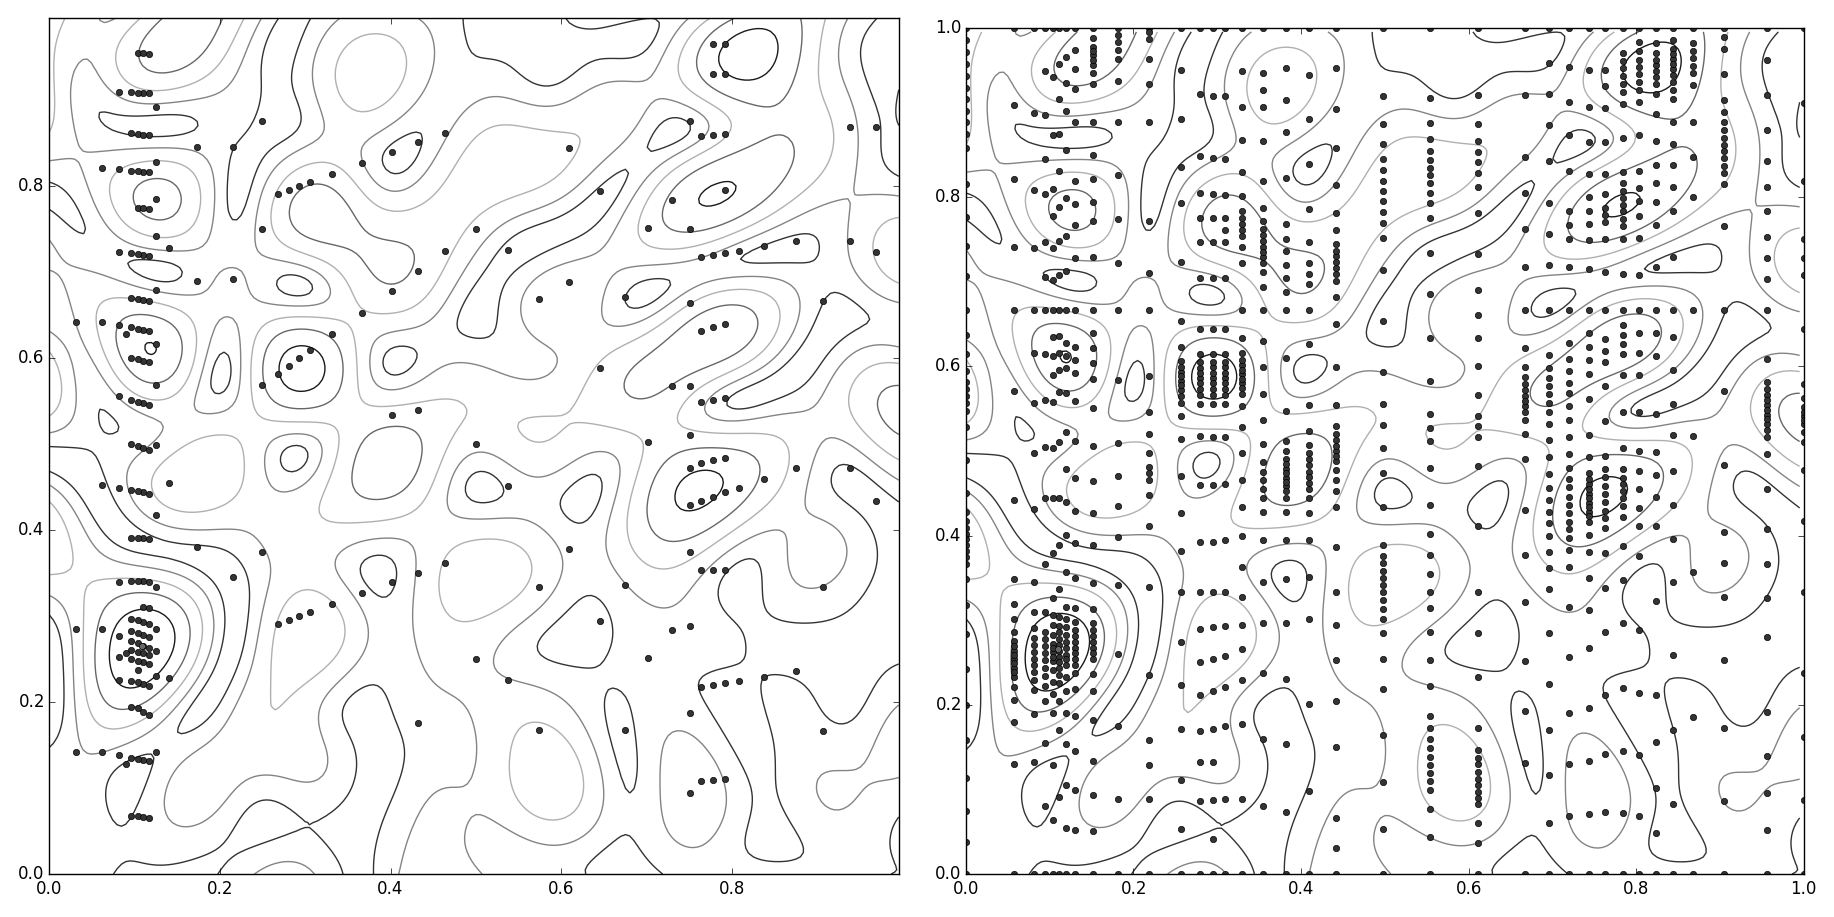
\includegraphics[width=116mm]{Fig2.png}
\caption{\label{fig:2}The placement of the trials by the adaptive scheme (the left panel) and by the basic one (the right panel).}
\end{figure}

The comparison of the efficiencies of the optimization algorithms using the examples of solving particular test problems, obviously, is not a sufficiently convincing way for proving the advantages of one or another method. Carrying out some multiple experiments in order to obtain the statistically reliable results of the comparison is a more objective approach. For this goal one can use the method of operating  characteristics introduced in \cite{Ref10, Ref36}.

The \textit{operating characteristic} is a set of pairs:
\begin{equation*}
\{ \langle k, p(k) \rangle \},
\end{equation*}
%
where $k$ is the number of search iterations and $p(k)$ is the number of the problems from the test class solved successfully in $k$ iterations. An individual pair corresponds to a particular set of the parameters of the method, which the test problems were solved by. Such indicators can be calculated according to the results of numerical experiments for various parameters of the methods and presented as a plot in the $(k, p)$ axes. If for a given value $k$ the operating characteristic of a method is situated  above the  characteristic of another method, the first method provides a better reliability, i.e., the possibility of the proper solution of the problem at the same computational costs for the search. If for a given value $p(k)$ the operating characteristic of a method is located on the left of the characteristic of another method, the first method requires less computational expenditures to achieve the same reliability. Thus, the operating characteristics allow comparing the efficiencies of various methods visually.

Let us first consider the class of two-dimensional functions~\ref{eq:30} consisting of $100$ functions. For a comparative experiment four global optimization methods have been taken. These are the basic nested optimization scheme (BS), the adaptive one (AS) and two methods based on other approaches to solving the global optimization problems: the partitioning method DIRECT (see~\cite{Ref17}) and the algorithm applying the dimensionality reduction by means of Peano mappings (PMA) from~\cite{Ref36}. In BS and AS the reliability parameter value $r = 2.6$ was used, for PMA $r = 3.2$ (these values provide sufficient conditions of convergence to global minimum for these methods). The operating characteristics have been obtained by varying the accuracy in the termination condition~\ref{eq:19} for AS, BS and PMA and the number of trials as the termination rule in DIRECT. The problem was considered to have been solved successfully if the coordinates of the minimal value found in the course of optimization are located in the circular neighborhood of the real minimum with the radius $0.01$. The results of the experiment are presented in Table~\origref{tab:1} and Fig.~\origref{fig:3}. The number of trials is plotted on the abscissa axis in the logarithmic scale.

\begin{table}[H]
\centering
\caption{\label{tab:1}The number of the problems solved successfully in dependence on trials spent.}
\begin{tabular}{|c|c|c|c|c|}
  \hline
  Number of trials &  AS &  BS & PMA & DIRECT \\ \hline
  60               &  40 &  42 &  25 & 13     \\ \hline
  100              &  51 &  61 &  52 & 31     \\ \hline
  150              &  72 &  73 &  71 & 52     \\ \hline
  200              &  87 &  84 &  80 & 66     \\ \hline
  250              &  88 &  87 &  88 & 75     \\ \hline
  300              &  89 &  90 &  92 & 83     \\ \hline
  400              &  94 &  94 &  96 & 89     \\ \hline
  500              &  99 &  96 &  96 & 92     \\ \hline
  700              & 100 &  98 &  97 & 94     \\ \hline
  800              & 100 &  99 &  99 & 97     \\ \hline
  1000             & 100 &  99 & 100 & 99     \\ \hline
  1100             & 100 & 100 & 100 & 100    \\ \hline
\end{tabular}
\end{table}

\begin{figure}[H]
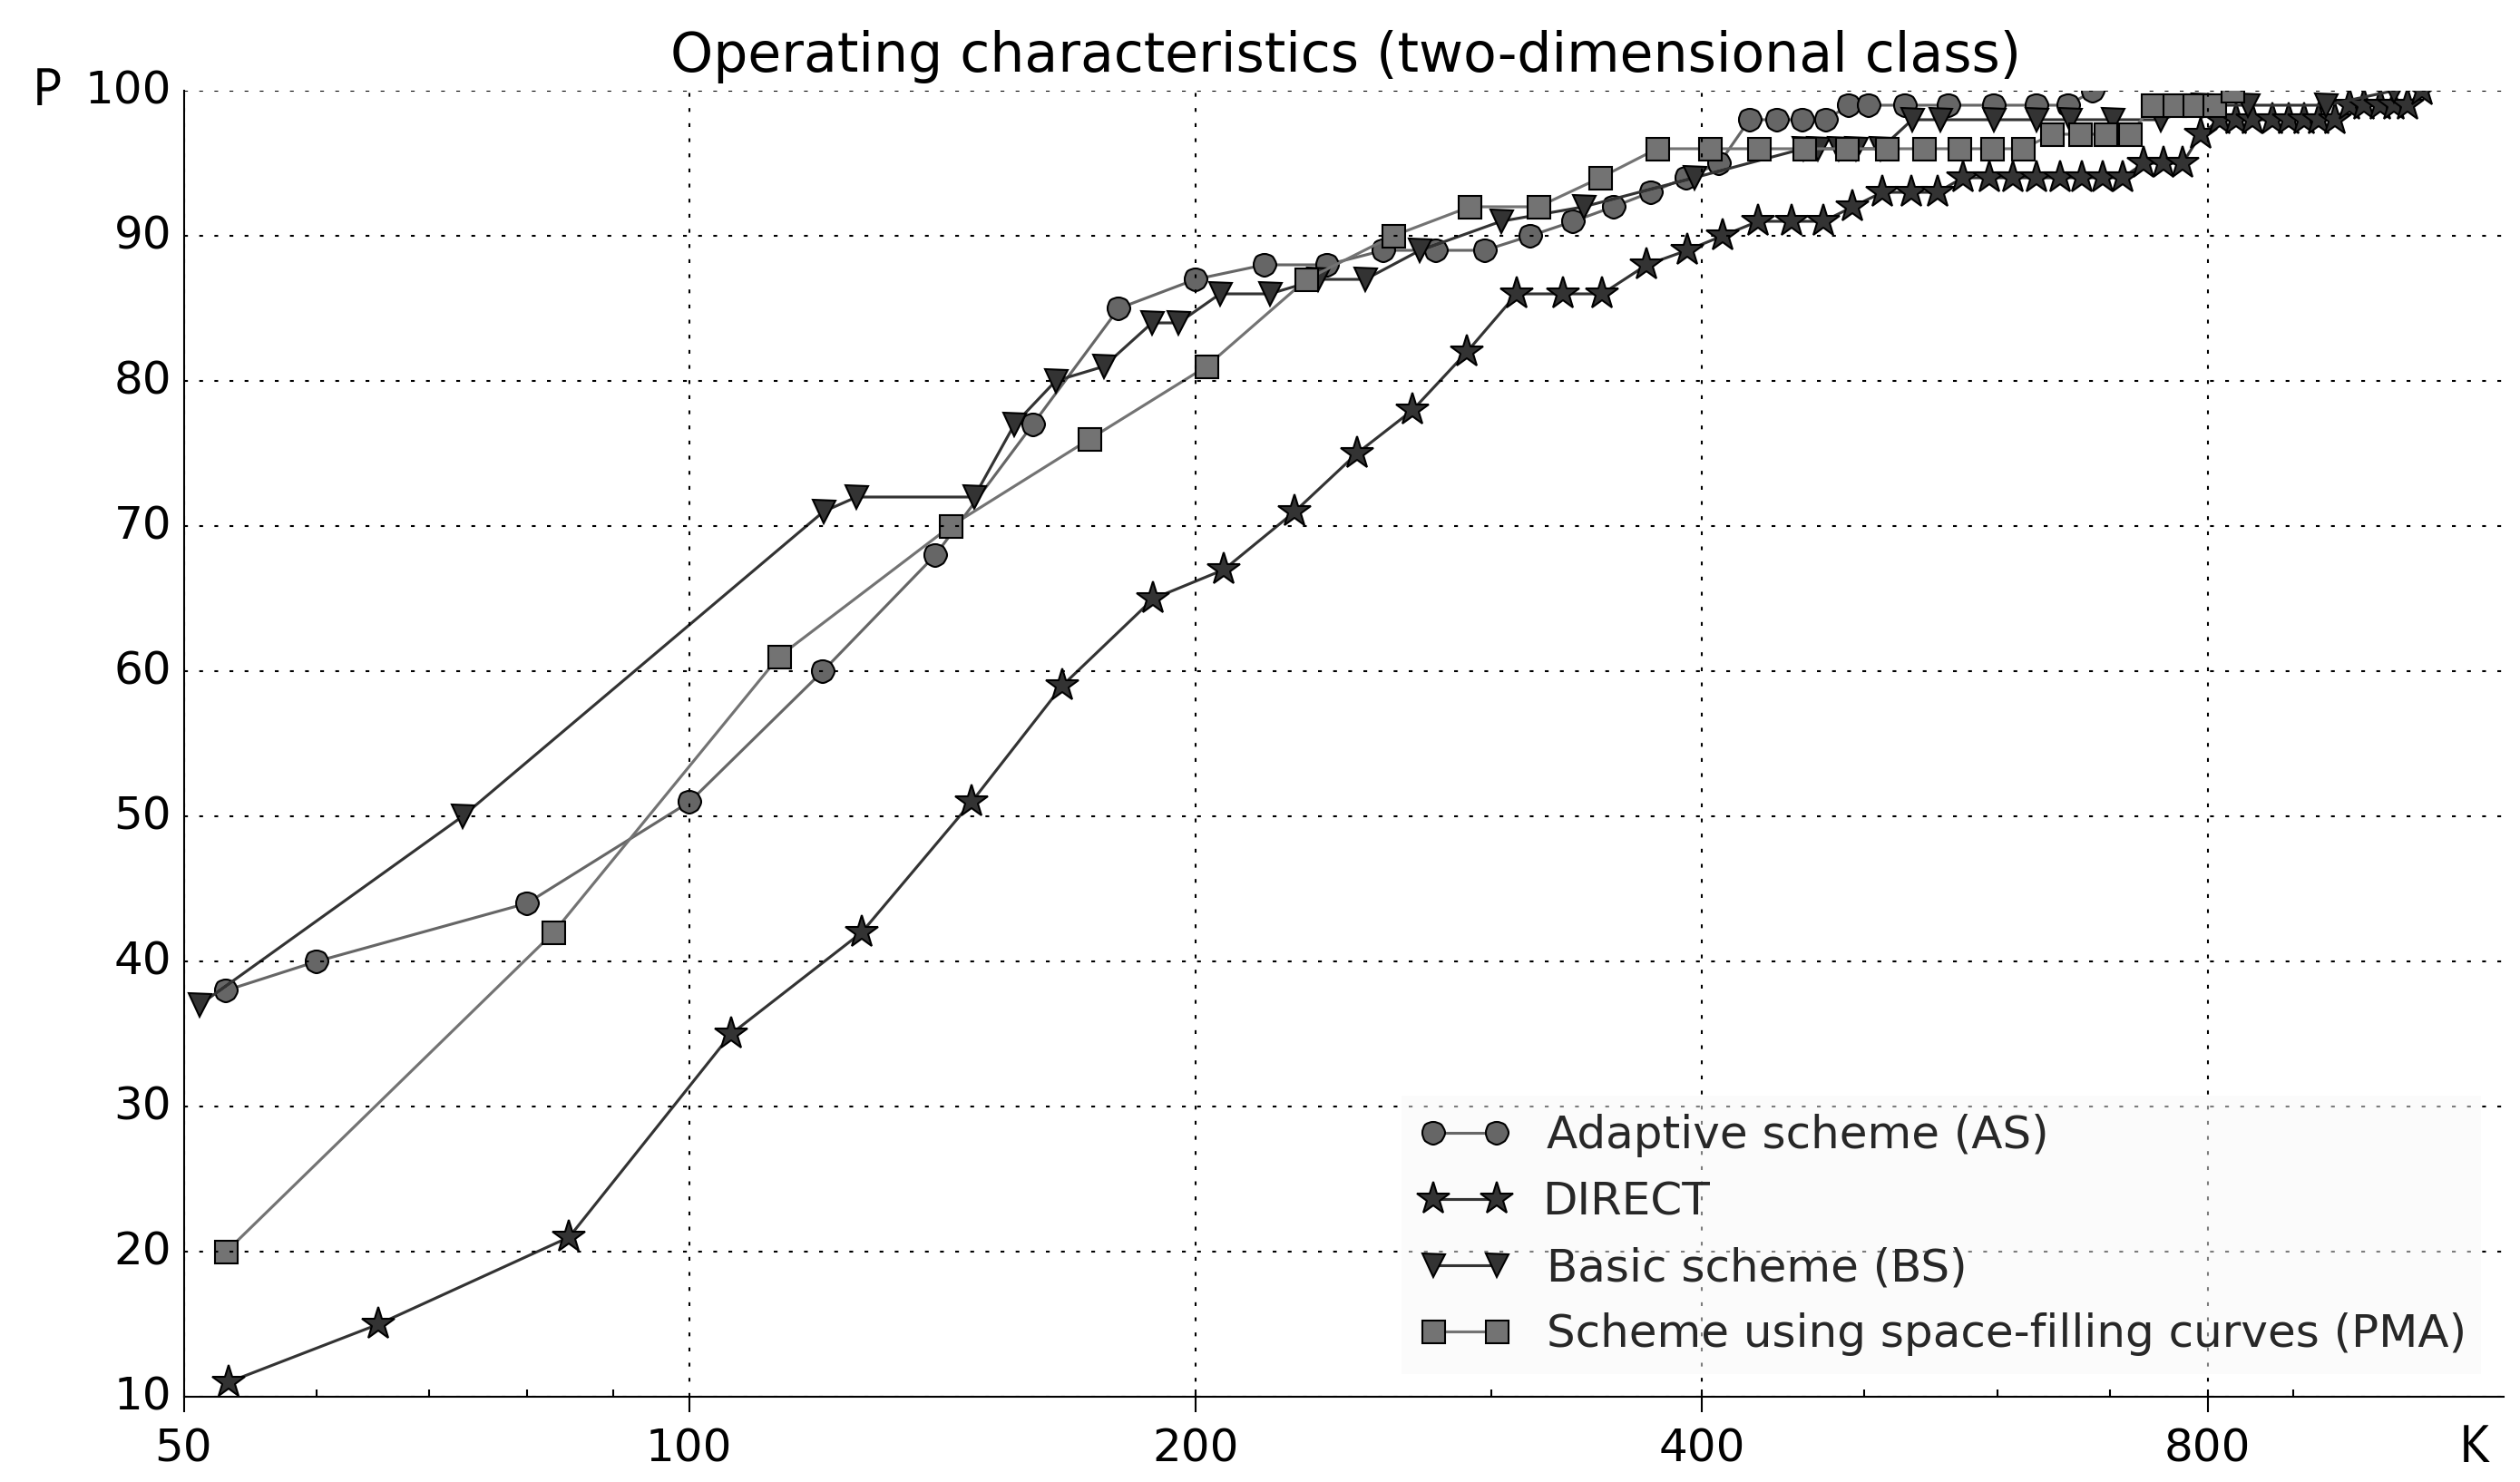
\includegraphics[width=120mm]{Fig3.png}
\caption{\label{fig:3}Operating characteristics on the class~\ref{eq:30}.}
\end{figure}

The numerical experiments have demonstrated an appreciable advantage of the adaptive scheme over the basic prototype and better performance of the adaptive scheme in providing a better reliability in comparison with the method DIRECT and the algorithm based on Peano curves.

The second series of the numerical experiments has been carried out using a well-known class of test functions GKLS from \cite{Ref6} for the 5-dimensional problems. The testing has been realized for a sample set of $100$ GKLS functions belonging to the most complicated GKLS class among the test classes described in~\cite{Ref6}.

Fig. \origref{fig:4} presents the operating characteristics for the basic nested optimization scheme (BS), the adaptive scheme (AS) and the Peano-mapping-based algorithm (PMA). All the methods used the value of parameter $r = 5$. The choice of the value $r = 5$ was caused by the necessity to satisfy the sufficient conditions of convergence for PMA. For this method, the inequality $m > 4L$ is the sufficient condition for the global convergence from \cite{Ref32}. The number of trials is plotted on the abscissa axis in the logarithmic scale.
\begin{figure}[H]
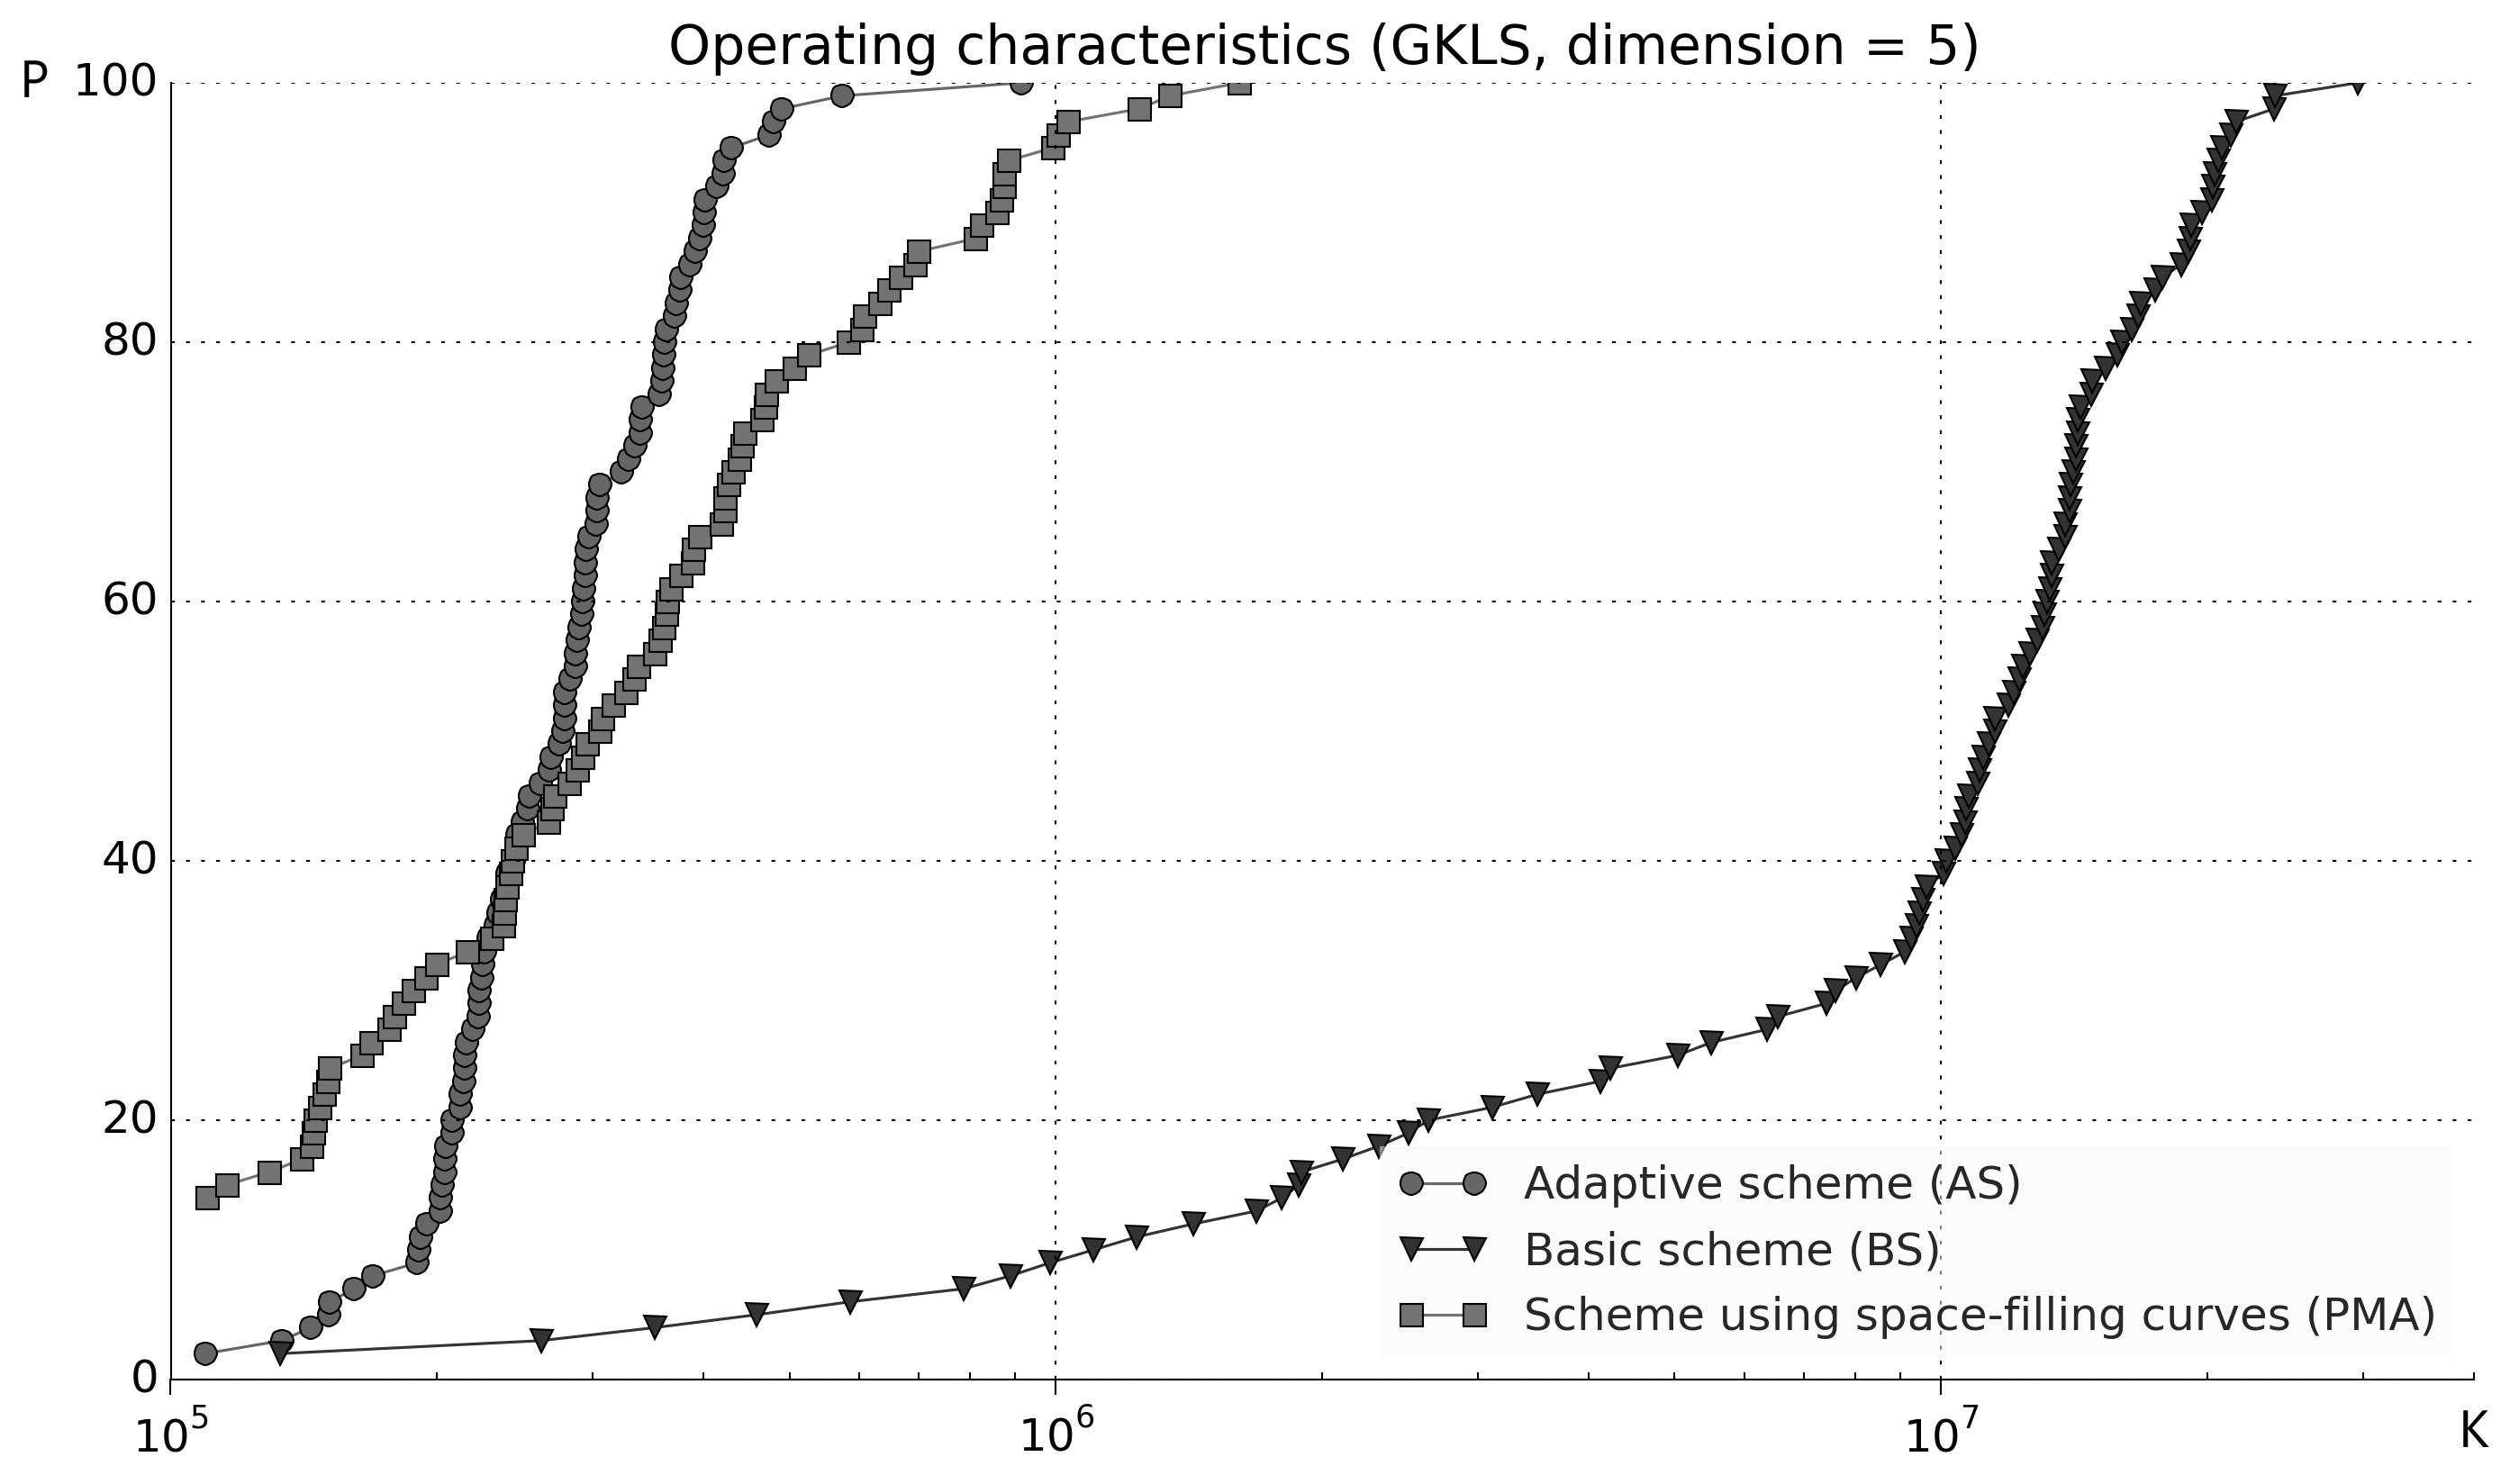
\includegraphics[width=116mm]{Fig4.png}
\caption{\label{fig:4}Operating characteristics using GKLS class.}
\end{figure}

As it follows from Fig. \origref{fig:4}, performance of the method BS is significantly worth than performance of the algorithms AS and PMA. The explanation of this fact consists in the phenomenon of the information loss by BS in the course of optimization as it was discussed above. Concerning the comparison of AS and PMA, one can note that for small number of iterations (and, as a result, for low reliability) the method using Peano  curves  has some  advantage. However, for achievement of a high reliability AS is more efficient than BS because it spends less number of trials.
\section{Conclusions}
\label{sec:7}
The work has been done in the framework of global optimization approach, according to which in order to construct the efficient global search algorithms, various dimensionality reduction schemes are applied. The reduction of the multidimensional problems to the one-dimensional ones allows using a wide choice of the one-dimensional algorithms to solve the multidimensional optimization problems.

In the present article, the nested optimization scheme of dimensionality reduction is considered. Along with a relative simplicity in its basic form, this scheme possesses a number of disadvantages including the redundancy of the number of computations of the minimized function values in the subdomains of the search domain. The authors have proposed a novel method to increase the efficiency of the initial scheme by means of using the full information on the problem in the course of global search. The novel adaptive scheme has been described in the generalized characteristic form, within the framework of which many one-dimensional global optimization algorithms can be employed. The generalized form has been specified for the case of the information global search method, which the proving of the convergence conditions has been done for. In order to confirm the efficiency of the developed approach, the results of the numerical experiments are presented justifying an essential acceleration of the search for the adaptive generalization as compared to the basic prototype and demonstrating the efficiency of the adaptive scheme as compared to the global optimization method based on application of Peano space-filling curves and to the popular method DIRECT.

It is worth noting that because of using the characteristic decision rule for selection of the coordinates for the next iteration, the adaptive scheme has a significant potential for the parallelization that may be a promising direction for its further development.

\begin{acknowledgements}
The authors thank Ruslan Israfilov for a significant contribution to computational experiments. The revised version of the paper was supported by the Russian Science Foundation, project  No. 15-11-30022 ``Global optimization, supercomputing computations, and applications''.
\end{acknowledgements}


\begin{thebibliography}{}
\bibitem{Ref1}
Butz, A.R.: Space-Filling Curves and Mathematical Programming. Inform. Control 12(4), 314--330 (1968)

\bibitem{Ref2}
Carr, C.R., Howe, C.W.: Quantitative Decision Procedures in Management and Economic: Deterministic Theory and Applications. McGraw–Hill, New York (1964)

\bibitem{Ref3}
Dam, E.R., Husslage, B., Hertog, D.: One-dimensional Nested Maximin Designs. Journal of Global Optimization 46(2), 287--306 (2010)

\bibitem{Ref4}
Floudas, C.A., Gounaris, C.E.: A Review of Recent Advances in Global Optimization. Journal of Global Optimization 45(1), 3--38 (2009)

\bibitem{Ref5}
Floudas, C.A., Pardalos, P.M., editors. Encyclopedia of Optimization. Kluwer Academic Publishers, Dordrecht (2001) (The 2nd ed. Springer, 2009)

\bibitem{Ref6}
Gaviano, M., Kvasov D.E., Lera D., Sergeyev Ya.D.: Software for generation of classes of test functions with known local and global minima for global optimization. ACM TOMS 29 (4), 469--480 (2003)

\bibitem{Ref7}
Gergel, V.P., Strongin, R.G.: Parallel computing for globally optimal decision making. Lecture Notes in Computer Science (including subseries Lecture Notes in Artificial Intelligence and Lecture Notes in Bioinformatics) 2763, 76-88 (2003)

\bibitem{Ref8}
Gergel, V., Grishagin, V., Israfilov R.: Local Tuning in Nested Scheme of Global Optimization. Procedia Computer Science 51, 865–874 (2015)

\bibitem{Ref9}
Goertzel, B.: Global Optimization with Space-Filling Curves. Applied Mathematics Letters 12(8), 133--135 (1999)`

\bibitem{Ref10}
Grishagin, V.A.: Operating Characteristics of Some Global Search Algorithms. Problems of Statistical Optimization 7, 198--206. Zinatne, Riga (1978) (In Russian)

\bibitem{Ref11}
Grishagin, V.A., Sergeyev, Y.D., Strongin, R.G.: Parallel Characteristic Algorithms for Solving Problems of Global Optimization. Journal of Global Optimization 10(2), 185--206 (1997)

\bibitem{Ref12}
Grishagin, V.A., Strongin, R.G.: Optimization of multiextremal functions subject to monotonically unimodal constraints. Engineering Cybernetics 5, 117--122 (1984)

\bibitem{Ref13}
Hime, A. E., Oliveira Jr., H.A., Petraglia, A.: Global Optimization Using Space-Filling Curves and Measure-Preserving Transformations. Soft Computing in Industrial Applications 96, 121--130 (2011)

\bibitem{Ref14}
Horst, R., Pardalos, P.M., editors.: Handbook of Global Optimization. Kluwer Academic Publishers, Dordrecht (1995)

\bibitem{Ref15}
Horst, R., Pardalos, P.M., Thoai, N.V.: Introduction to Global Optimization. Kluwer Academic Publishers, Dordrecht (1995). (2nd ed. Kluwer Academic Publishers, 2001).

\bibitem{Ref16}
Horst, R., Tuy, H.: Global Optimization: Deterministic Approaches. Springer-Verlag, Berlin (1990)

\bibitem{Ref17}
Jones, D.R.: The DIRECT Global Optimization Algorithm. In: Floudas C.A., Pardalos P.M. (eds) Encyclopedia of optimization 1. Kluwer Academic Publishers, Dordrecht, 431--440 (2001)

\bibitem{Ref18}
Kushner, H.J.: A new method of locating the maximum point of an arbitrary multipeak curve in the presence of noise. Transactions of ASME, Ser. D. Journal of Basic Engineering 86, 1, 97--106 (1964)

\bibitem{Ref19}
Kvasov, D.E., Pizzuti, C., Sergeyev, Y.D.: Local tuning and partition strategies for diagonal GO methods. Numerische Matematik 94(1),  93--106  (2003)

\bibitem{Ref20}
Kvasov, D.E., Sergeyev, Ya.D.: Multidimensional Global Optimization Algorithm Based on Adaptive Diagonal Curves. Comput. Math. Math. Phys. 43(1), 40--56 (2003)

\bibitem{Ref21}
Kvasov, D.E., Sergeyev, Y.D.: Lipschitz gradients for global optimization in a one-point-based partitioning scheme.  Journal of Computational and Applied Mathematics  236(16),  4042--4054 (2012)

\bibitem{Ref22}
Kvasov, D.E., Sergeyev, Ya.D.: Deterministic approaches for solving practical black-box global optimization problems. Advances in Engineering Software 80, 58-66 (2015)

\bibitem{Ref23}
Paulavicius, R., Sergeyev, Y.D., Kvasov, D.E., Zilinskas, J.: Globally-biased DISIMPL algorithm for expensive global optimization. Journal of Global Optimization 59(2--3), 545--567 (2014)

\bibitem{Ref24}
Pintér, J. D.: Global Optimization in Action (Continuous and Lipschitz Optimization: Algorithms, Implementations and Applications). Kluwer Academic Publishers, Dordrecht (1996)

\bibitem{Ref25}
Piyavskij, S.A.: An Algorithm for Finding the Absolute Extremum of a Function. USSR Comput. Math. Math. Phys. 12(4), 57--67 (1972)

\bibitem{Ref26}
Sergeyev, Y.D., Grishagin V.A.: A Parallel Method for Finding the Global Minimum of Univariate Functions. Journal of Optimization Theory and Applications  80(3), 513--536 (1994)

\bibitem{Ref27}
Sergeyev, Y.D.: An efficient strategy for adaptive partition of N-dimensional intervals in the framework of diagonal algorithms. Journal of Optimization Theory and Applications 107(1), 145-168 (2000).

\bibitem{Ref28}
Sergeyev, Y.D., Grishagin, V.A.: Parallel Asynchronous Global Search and the Nested Optimization Scheme. J. Comput. Anal. Appl.  3(2), 123--145 (2001)

\bibitem{Ref29}
Sergeyev Ya.D.: Efficient partition of N-dimensional intervals in the framework of one-point-based algorithms. Journal of Optimization Theory and Applications, 124(2), 503-510 (2005).

\bibitem{Ref30}
Sergeyev, Ya. D., Strongin, R. G., Lera, D.: Introduction to Global Optimization Exploiting Space-Filling Curves. Springer (2013)

\bibitem{Ref31}
Shi, L., Ólafsson, S.: Nested Partitions Method for Global Optimization. Operations Research 48(3), 390--407 (2000)

\bibitem{Ref32}
Shubert, B.O.: A Sequential Method Seeking the Global Maximum of a Function. SIAM Journal on Numerical Analysis 9(3), 379--388 (1972)

\bibitem{Ref33}
Strekalovsky, A.S.: On Solving Optimization Problems with Hidden Nonconvex Structures. In: Rassias Th.M., Floudas Ch.A., Butenko S. (eds) Optimization and Science in Engineering. Springer, 465-502 (2014)

\bibitem{Ref34}
Strongin, R.G.: Numerical Methods in Multiextremal Problems (Information-Statistical Algorithms). Nauka, Moscow (1978). (In Russian)

\bibitem{Ref35}
Strongin, R.G.: The information approach to multiextremal optimization problems. Stochastics and Stochastic Reports 27, 65--82 (1989)

\bibitem{Ref36}
Strongin, R.G., Sergeyev, Ya.D.: Global Optimization with Non-convex Constraints: Sequential and Parallel Algorithms. Kluwer Academic Publishers, Dordrecht (2000, 2nd ed. 2013, 3rd ed. 2014)

\bibitem{Ref37}
Törn, A., Žilinskas, A.: Global Optimization. Lecture Notes in Computer Science 350. Springer-Verlag, Berlin (1989)

\bibitem{Ref38}
Zhigljavsky, A.A.: Theory of Global Random Search. Kluwer Academic Publishers, Dordrecht (1991)

\bibitem{Ref39}
Zhigljavsky, A.A., Chekmasov, M.V.: Comparison of independent, stratified and random covering sample schemes in optimization problems. Mathematical  and Computer Modelling  23(8--9), 97--110 (1996)
\end{thebibliography}

\end{document}
